\documentclass[USenglish,pdftex,compress,10pt,svgnamesi,handout]{beamer}
%\documentclass[USenglish,pdftex,compress,10pt,svgnames]{beamer}
%\documentclass[notes,10pt,svgnames]{beamer}
\usepackage{import}\subimport{../../common/}{lectureheader}

\graphicspath{{pics/}}
\usepackage{listings}

\parskip2ex
\usepackage{tabu}

\newcommand{\bfw}{\Vec{w}}
\newcommand{\bfx}{\Vec{x}}
\newcommand{\bfz}{\Vec{z}}
\newcommand{\bfg}{\Vec{g}}
\newcommand{\bfu}{\Vec{u}}
\def\bf#1{\Vec{#1}}
\def\cl#1{{\cal #1}}
\DeclareMathOperator{\sgn}{sgn}
\def\hid{{H}}

\usepackage{movie15}

% =====================================================================
% Titel etc.
\hypersetup{%
	pdftitle={neural networks: practical considerations},%
	pdfauthor={Patrick van der Smagt}%
}

\title{neural networks: practical considerations}
\author{Patrick van der Smagt}
\date{}
% =====================================================================
\begin{document}


%'''''''''''''''''''''''''''''''''''''''''''''''''''''''''
\begin{frame}
	\titlepage
	
	\vfil
\end{frame}


\begin{frame}
\frametitle{some good and some bad news}
\hfill
\begin{beamerboxesrounded}[scheme=proof,width=0.95\textwidth,shadow=true]{\textbf{universal approximation}}
	an MLP with at least two layers of weights can approximate arbitrarily well any given mapping from one finite input space with a finite number of discontinuities to another, if we have enough hidden units [Cybenko 1989; Funahashi 1989; Hornik et al 1989, 1991; Hartman et al 1990].
\end{beamerboxesrounded}
\hspace*{\fill}
\bigskip
	\pause

\hfill
\begin{beamerboxesrounded}[scheme=proof,width=0.95\textwidth,shadow=true]{\textbf{parameter finding}}
	finding the optimum set of weights $\bfw$  for an MLP is an NP-complete problem, i.e.\ it cannot be solved exactly within a time $t\propto |\bfw|^x$ [Blum et al., 1992].
\end{beamerboxesrounded}
\hspace*{\fill}
\end{frame}





%%%%%%%%%%%%%%%%%%%%%%%%%%%%%%%%%%%%
%%%%%%%%%%%%%%%%%%%%%%%%%%%%%%%%%%%%
%%%%%%%%%%%%%%%%%%%%%%%%%%%%%%%%%%%%
%%%%%%%%%%%%%%%%%%%%%%%%%%%%%%%%%%%%
%%%%%%%%%%%%%%%%%%%%%%%%%%%%%%%%%%%%
%%%%%%%%%%%%%%%%%%%%%%%%%%%%%%%%%%%%
%%%%%%%%%%%%%%%%%%%%%%%%%%%%%%%%%%%%
%%%%%%%%%%%%%%%%%%%%%%%%%%%%%%%%%%%%







%\frame{\frametitle{options for regularising neural networks}
%\begin{tabular}{ll}
%	\textbf{Modification} & \textbf{Issues} \\\hline
%	use \alert{small enough} network & $\ominus$ loses generalisation capabilities\\[2mm]
%	\pause
%	early stopping & $\ominus$ need extra data for testing\\
%	& $\ominus$ which data to choose for cross-validation?\\[2mm]
%	\pause
%	introduce \alert{weight decay} term & $\ominus$ weights are regularised towards 0!\\[2mm]
%	add Gaussian noise to inputs & $\ominus$ is it realistic?  \\
%	& $\ominus$ increases training time\\[2mm]
%	\pause
%	full Bayesian treatment & $\ominus$ nonlinear transfer functions prohibit that
%\end{tabular}
%}
%
%
%



\begin{frame}
\frametitle{how did deep learning evolve?}

In the 1990's, FFNN's have been used in many areas, including process control, classification, stock exchange prediction, diagnosis, robot control, sensory data fusion, etc. But they did not live up to their expectation, and after their hype (1986--1995) they lost in popularity.  

In fact, their restricted representation and generalisation properties was one of the biggest problems.

$\rightarrow$ IEEE journals, ICML had policies not to accept NN papers

Recent results with deep neural networks have shown that the don't-give-up approach can give great results.  Neural networks now can be used to solve real-world problems (google speech recognition, Street View house number recognition, image recognition, \dots)
\end{frame}




% use this for invisible text, in particular invisible underbraces
\def\i#1{\textcolor{white}{#1}}

%% vanishing gradient
\begin{frame}<handout:0>
\frametitle{a big problem: the vanishing gradient}
It is usually true that 
$$  \partial E(\bfw) / \partial w_{ij}^{(\hid)}
  \gg
    \partial E(\bfw) / \partial w_{ij}^{(\hid-1)}
$$
i.e., the lower you get in the network, the more the gradient vanishes.

After all,
$$
{\partial E(\bfw)  \over \partial w_{ij}^{(\hid-1)} }
    = \delta^{(\hid-1)}_j x_i 
    = \sum_l \i{\underbrace{\textcolor{black}{\delta_l^{(\hid)}}}_{\mathrm{small}}}
    	\i{\underbrace{{}_l^(}_{\i{\times}}}
	\i{\underbrace{ \textcolor{black}{w_{lk}^{\i(} x_i }}_{\mathrm{small}}}
	\i{\underbrace{=smaller_l^(}_{=\,\,\,\mathrm{smaller!}}} 
$$\end{frame}

\begin{frame}
\frametitle{a big problem: the vanishing gradient}
It is usually true that 
$$  \partial E(\bfw) / \partial w_{ij}^{(\hid)}
  \gg
    \partial E(\bfw) / \partial w_{ij}^{(\hid-1)}
$$
i.e., the lower you get in the network, the more the gradient vanishes.

After all,
$$
{\partial E(\bfw)  \over \partial w_{\hid-1,i,j} }
    = \delta_{\hid-1,j} x_i 
    = \sum_l {\underbrace{\textcolor{black}{\delta_{\hid,l}}}_{\mathrm{small}}}
    	\i{\underbrace{{}_l^(}_{\textcolor{black}{\times}}}
	{\underbrace{ \textcolor{black}{w_{Hlk} x_i }}_{\mathrm{small}}}
	\i{\underbrace{=smaller_l^(}_{\textcolor{black}{=\,\,\,\mathrm{smaller!}}}}
$$\end{frame}







\begin{frame}
\frametitle{$E($XOR$)$, 1 hidden layer}
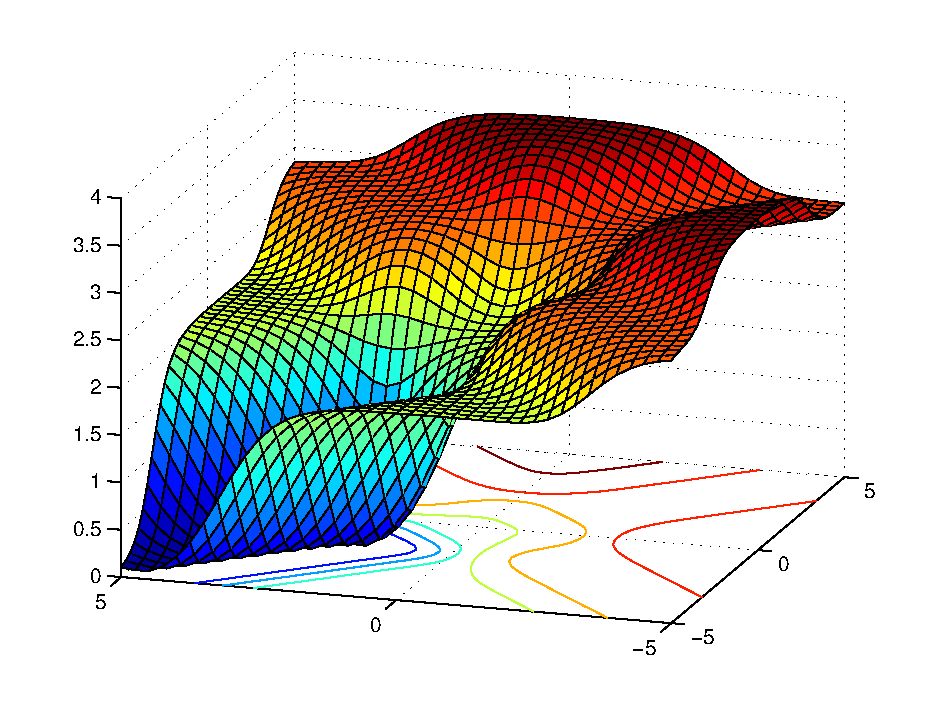
\includegraphics[width=6cm]{pics/xor_in1_1hidden}
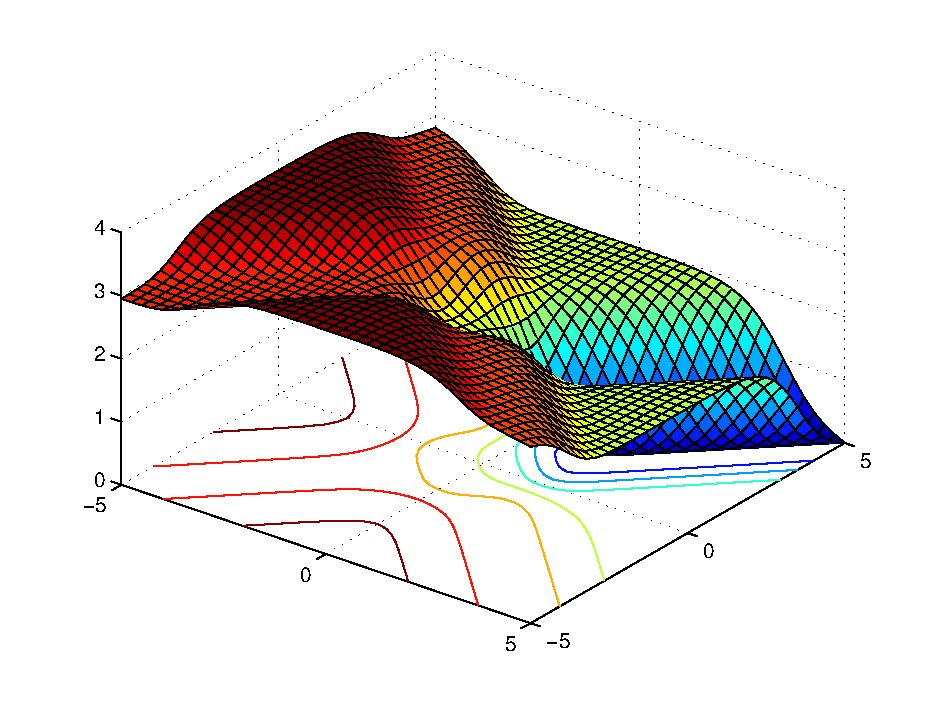
\includegraphics[width=6cm]{pics/xor_in2_1hidden}

$E(\Vec w_1)$
\end{frame}



\begin{frame}
\frametitle{$E($XOR$)$, 3 hidden layers}
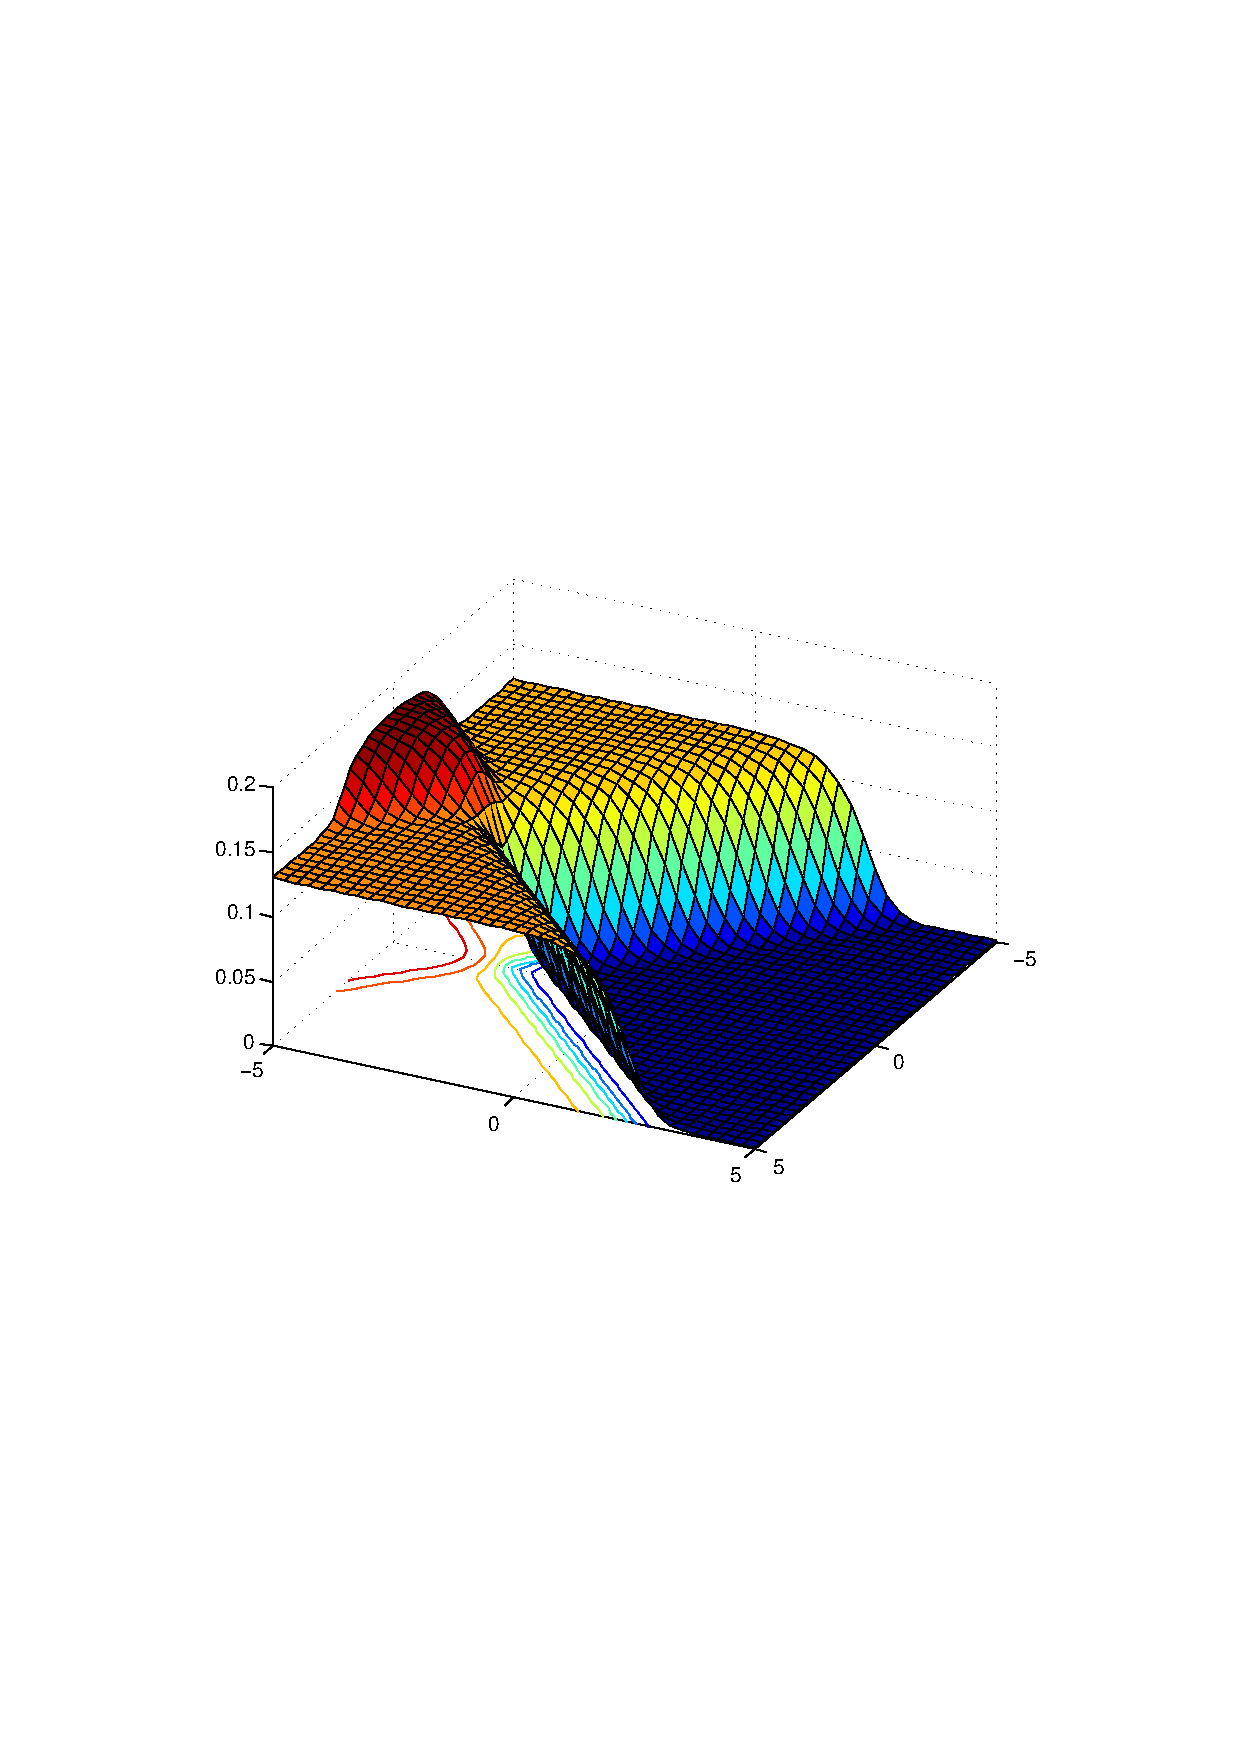
\includegraphics[width=6cm]{pics/xor_in1_3hidden}
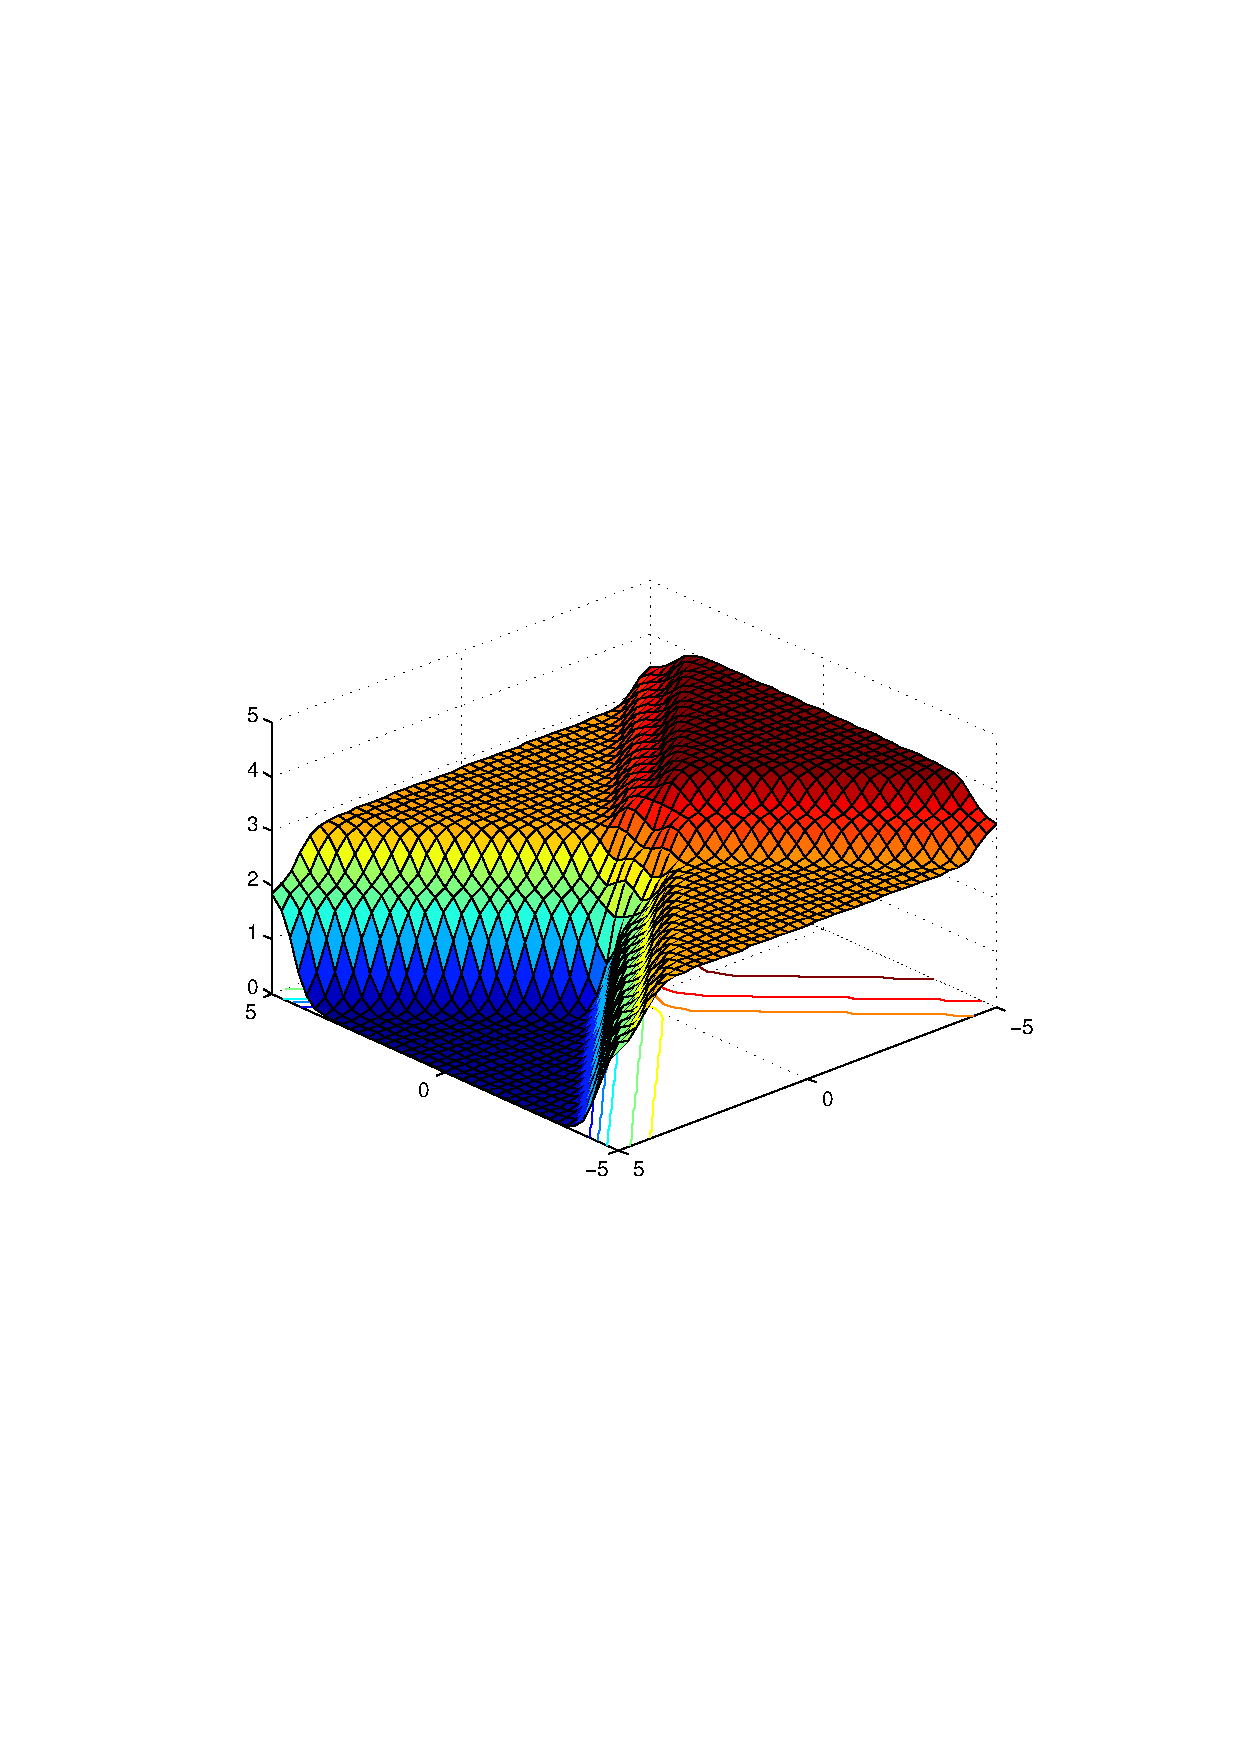
\includegraphics[width=6cm]{pics/xor_in2_3hidden}

$E(\Vec w_1)$
\end{frame}


\begin{frame}
\frametitle{$E($XOR$)$, 10 hidden layers}
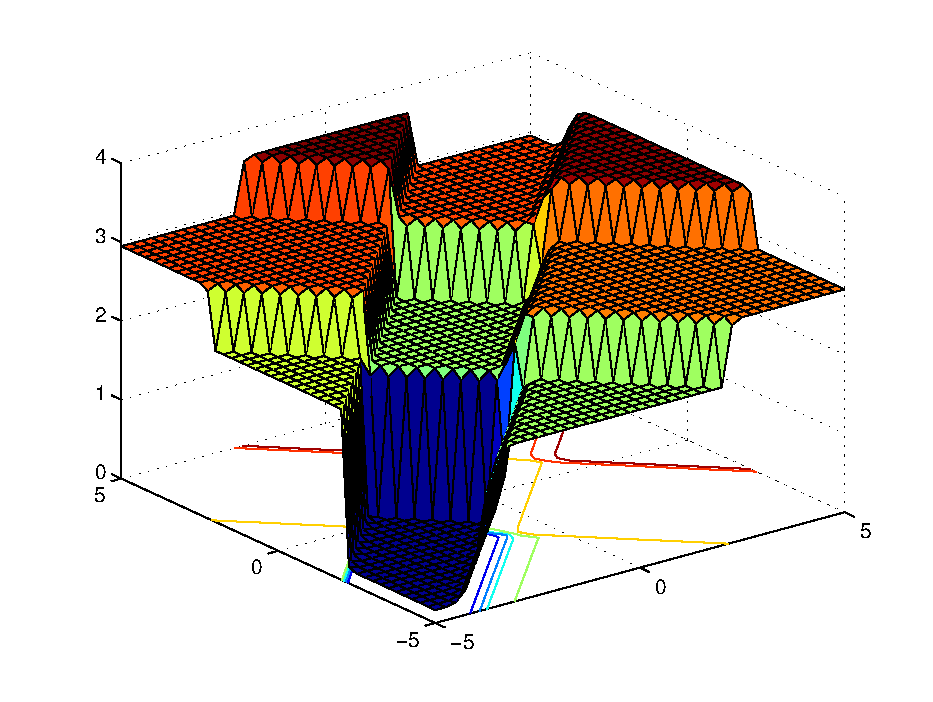
\includegraphics[width=6cm]{pics/xor_in1_10hidden}
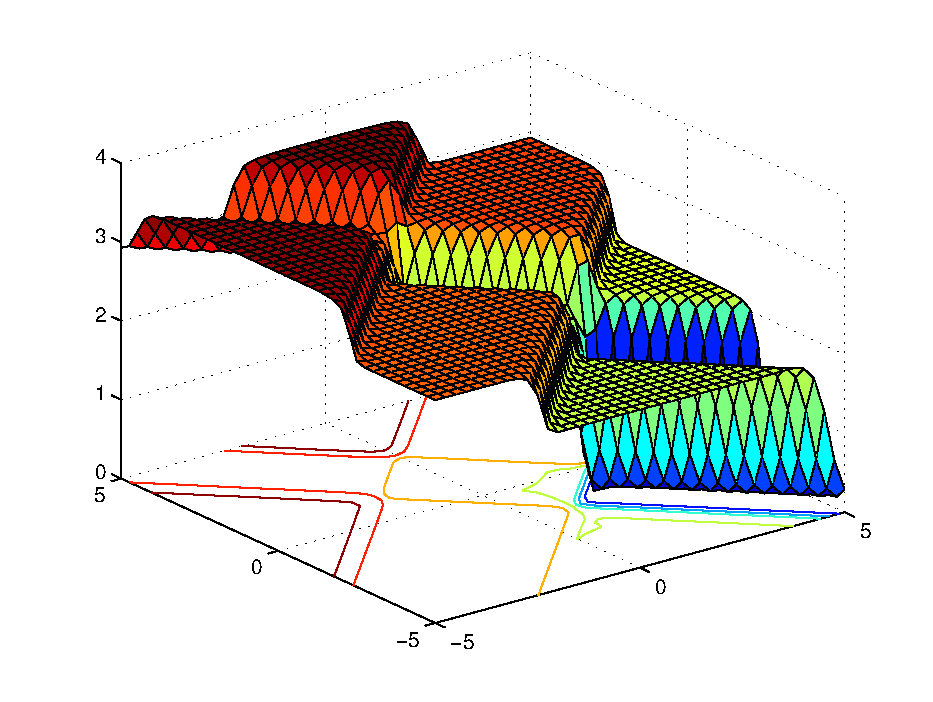
\includegraphics[width=6cm]{pics/xor_in2_10hidden}

$E(\Vec w_1)$
\end{frame}




\begin{frame}
\frametitle{way out}
Back-propagation is difficult for multiple hidden layers due to the vanishing gradient.

Unsupervised pretraining with \textsl{Restricted Boltzmann Machines} (Hinton et al., 2006) solved that.

However, it was later found that DNN can also be successfully  trained:
\begin{itemize}
  \item use many labelled data (e.g., now well possible for images);
  \item train ``longer'' (possible with GPUs);
  \item better weight initialisation (new methods were developed);
  \item regularise with ``batch normalisation'' or ``layer normalisation'' or ``dropout''.
\end{itemize}

Sometimes the use of rectified linear units $\max(0,x)$ or $\log(1+e^x)$ improve things, too.

\end{frame}


\begin{frame}
\frametitle{why do multiple hidden layers improve generalisation?}

\begin{columns}
\begin{column}{0.6\textwidth}
Functions compactly represented with $k$ layers may require
exponential size with $k-1$ layers.
\vskip2ex

Multiple levels of latent variables allow combinatorial sharing
of statistical strength. 
\vskip2ex

Different high-level features share lower-level features.
\end{column}
\begin{column}{0.4\textwidth}
\vskip1cm
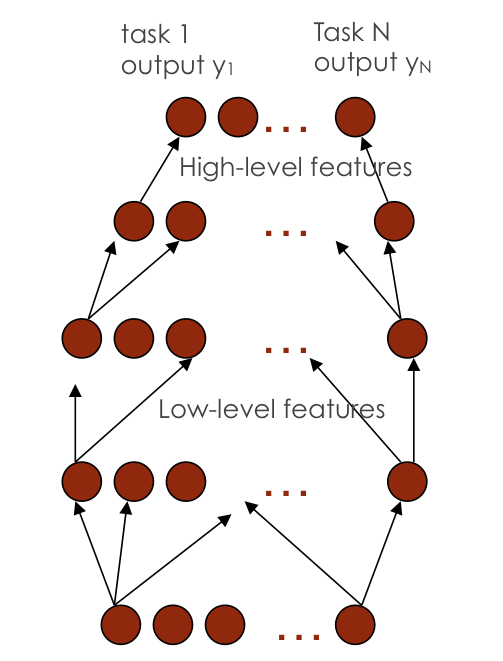
\includegraphics[width=\textwidth]{pics/bengio1.png}
\end{column}
\end{columns}

\footnotesize{from:
\emph{Understanding and Improving Deep Learning Algorithms},
Yoshua Bengio, ML Google Distinguished Lecture, 2010}
\end{frame}



%\begin{frame}
%\frametitle{back-propagation problems for deep networks}
%
%\begin{itemize}
%\item requires many labeled training data \\
%	\textcolor{white}{(yet since 1995 we have much bigger labeled data sets)}
%\item learning time does not scale well for multiple hidden layers\\
%	\textcolor{white}{(and computers became MUCH faster by GPUs)}
%\item initialising weights is important \\
%	\textcolor{white}{(so new methods were developed)}
%\end{itemize}
%\end{frame}
%

%\begin{frame}
%\frametitle{back-propagation problems for deep networks}
%
%\begin{itemize}
%\item requires many labeled training data \\
%	(yet since 1995 we have much bigger labeled data sets)
%\item learning time does not scale well for multiple hidden layers\\
%	 (and computers became MUCH faster by GPUs)
%\item initialising weights is important \\
%	(so new methods were developed)
%\end{itemize}
%\end{frame}

%%%%%%%%%%%%



%\vspace{1cm}
%
%Recent research [Hinton et al., 2006] uses 
%\emph{unsupervised pre-training} by Restricted 
%Boltzmann Machines to get into vicinity of the minimum.
%
%\vspace{1cm}
%
%Various kinds of unsupervised pre-training:
%\begin{itemize}
%\item RBM (Restricted Boltzmann Machines)
%\item (tied) Autoencoders and variants (denoising AE, sparse AE)
%\item Sparse coding
%\item \dots
%\end{itemize}
%\end{frame}
%
%
%\begin{frame}
%\frametitle{restricted Boltzmann machine}
%Start by learning a generative model of the input data that has one layer of latent variables
%\vskip1cm
%\centerline{\includegraphics[width=6cm]{pics/RBM.pdf}}
%
%Then use the vector of latent variable activities as data for training a second generative model.
%
%\end{frame}
%
%
%\begin{frame}
%\frametitle{restricted Boltzmann machine}
%for a hidden unit $h$ and a visible unit $v$ (bias $b$, weight $w$) we compute
%$$
%P(h_j = 1 \mid v) = \sigma \bigl(b_j + \sum_{i=1}^m w_{i,j} v_i \bigr), \quad  \textrm{$\sigma$ is sigmoid function}
%$$
%$$
%P(v_i= 1 \mid h) = \sigma \bigl(a_i + \sum_{j=1}^n w_{i,j} h_j \bigr), \quad  \textrm{\textcolor{white}{,s is sigmoid function}}
%$$
%we optimise
%$
%\argmax_W \prod_{v \in V} P(v)
%$
%e.g.\ using contrastive divergence:
%\pause
%\centerline{\includegraphics[width=6cm]{pics/contrastivedivergence.png}}
%
%\end{frame}
%
%
%\begin{frame}
%\frametitle{pretraining with RBMs}
%We can combine the stack of generative models into one.  We can prove that adding a layer results in a lower bound on the log probability of the training data.
%
%Then add an output layer, and train the stack with back propagation.
%\end{frame}
%
%
%\begin{frame}
%\frametitle{loose remarks}



\begin{frame}
\frametitle{rectifier linear units}

Here is a trick to make logistic neurons more powerful, but keeping the number of parameters constant:
\begin{enumerate}
\item make many copies of each neuron
\item all neurons have the same parameters, but have a fixed offset to the bias: $-1$, $-0.5$, $0.5$, \dots
\end{enumerate}

\begin{tabular}{ccc}
{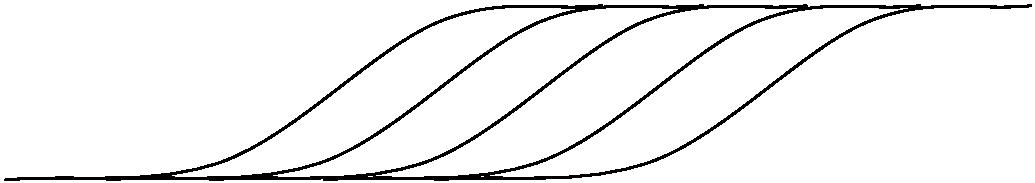
\includegraphics[width=5cm]{pics/sumlog.pdf}}
&=&
{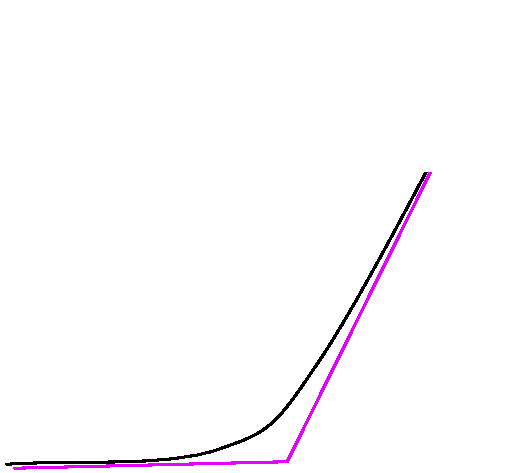
\includegraphics[width=3cm]{pics/rect.pdf}}
\\
&&\\
$\sum_{n=1}^\infty \mathrm{logistic}(x + 0.5 - n)$
&$\approx$&
$\log(1 + e^x)$
\end{tabular}
\vskip1cm
Apart from saving parameters, this also reduces the vanishing gradient.

(but there is no guarantee that this improves things)
\end{frame}


\begin{frame}
\frametitle{dropout}
Let's look at a neural network with one hidden layer.

Each time a learning sample is learned, we randomly put to 0 each hidden unit with probability 0.5.

\centerline{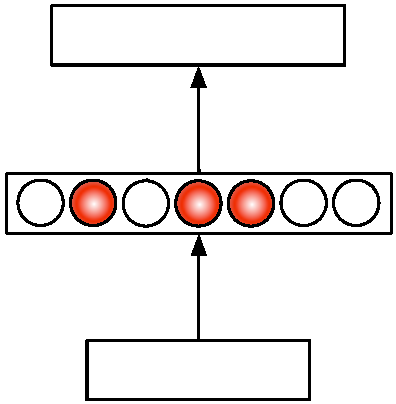
\includegraphics[width=4cm]{pics/dropout.pdf}}

We are therefore randomly sampling from $2^H$ different architectures, but these share the same weights.

\note{
Weight sharing means strong regularisation.
It is much better than L1 or L2 regularisation which pull the weights to 0; instead, it pulls the weights to what other models want.
}
\end{frame}


\begin{frame}
\frametitle{dropout: how is the output computed?}
To compute the output, one could average all possible models.

That is too expensive, however.  

Instead we take the half of the outgoing weights to get the same results.\\
This  computes the geometric mean of the predictions of all $2^H$ models.

\vfill

\begin{beamerboxesrounded}[scheme=proof,width=0.95\textwidth,shadow=true]{\textbf{Quote}}
	if your deep neural network is overfitting, use dropout. \\ If it isn't, it will probably be too small!.
\end{beamerboxesrounded}

\end{frame}





\begin{frame}[fragile]
\frametitle{algorithm for backprop (``on-line'' aka ``stochastic'' learning)}

\begin{beamerboxesrounded}[upper=def,lower=block body,width=1.03\textwidth,shadow]{\textbf{back-propagation algorithm:}}
\begin{lstlisting}[mathescape]
initialise the weights
repeat
  for each training sample $(\bfx,\bfz)$ do
  begin
     $\bf o = \cl M(\bfw, \bfx)$; forward pass
     calculate error $\bfz  - \bf o$ at the output units
     for all $w^{(2)}$ compute $\delta_{w^{(2)}}$; backward pass
     for all $w^{(1)}$ compute $\delta_{w^{(1)}}$; backward pass continued
     update the weights using $\partial E / \partial w_{ij} = \delta_{j} \phi'(\cdot) x_{i}$
  end
  (this is called one epoch)
until stopping criterion satisfied
\end{lstlisting}
\end{beamerboxesrounded}
What is wrong with this learning method?

\end{frame}





%%%%
\begin{frame}[fragile]
\frametitle{better algorithm for backprop (``(mini) batch learning'')}

\begin{beamerboxesrounded}[upper=def,lower=block body,width=1.03\textwidth,shadow]{\textbf{back-propagation algorithm:}}
\begin{lstlisting}[mathescape]
initialise the weights
repeat
  randomly select samples $(\bfx,\bfz)$ from a mini-batch do
  begin
     $\bf o = \cl M(\bfw, \bfx)$; forward pass
     calculate error $\bfz  - \bf o$ at the output units
     for all $w^{(2)}$ compute $\delta_{w^{(2)}}$; backward pass
     for all $w^{(1)}$ compute $\delta_{w^{(1)}}$; backward pass continued
     sum the delta weights using $\partial E / \partial w_{ij} = \delta_{j} \phi'(\cdot) x_{i}$
  end
  update the weights using summed delta weights
until stopping criterion satisfied
\end{lstlisting}
\end{beamerboxesrounded}
\textcolor{white}{What is wrong with this learning method?}

\end{frame}



\begin{poll}
The above algorithm computes an error $e_n = \bigl(\target_n - y(\Vec x_n, \Vec w)\bigr)^2$ and then updates the weights.

The formula however says the error equals $E = \sum_{n=1}^N \bigl(\target_n - y(\Vec x_n, \Vec w)\bigr)^2$.

Which statements are true?

\begin{enumerate} [A]
\item 
  It makes no difference, they are the same
\item
 It should instead compute $E = \sum_{n=1}^N \bigl(\target_n - y(\Vec x_n, \Vec w)\bigr)^2$
\item
 It is computationally cheaper as it need not evaluate $E$ for all data
\item
 It is computationally more expensive as it must update for each sample
\end{enumerate}
\end{poll}

%%%%%%%%%%%%%%





%
%\begin{frame}
%\frametitle{stochastic gradient descent}
%If the dataset is highly redundant, the gradient on the first half is almost identical to the gradient on the second half.
%\begin{itemize}
%\item So instead of computing the full gradient, update the weights using the gradient on the first half and then get a gradient for the new weights on the second half.
%\item  The extreme version of this approach updates weights after each case. It is called ``online.''
%\end{itemize}
% Mini-batches are usually better than online:
%\begin{itemize}
%\item Less computation is used updating the weights.
%\item Computing the gradient for many cases simultaneously uses matrix-matrix multiplies which are very efficient, especially on GPUs
%\end{itemize}
% Mini-batches need to be balanced for classes!
%\end{frame}
%
%










\begin{frame}
\frametitle{initialising the weights}
If two hidden units have exactly the same bias and exactly the same incoming and outgoing weights, they will always get exactly the same gradient.
\begin{itemize}
\item  So they can never learn to be different features.
\item  We break symmetry by initialising the weights to have small random values.
\end{itemize}
If a hidden unit has a big fan-in, small changes on many of its incoming weights can cause the learning to overshoot.
\begin{itemize}
\item  We generally want smaller incoming weights when the fan-in is big, so initialise the weights to be proportional to $\sqrt(\textrm{fan-in})$.
\end{itemize}
We can also scale the learning rate the same way.
\end{frame}




\begin{frame}
\frametitle{shifting the inputs}
\begin{columns}
\begin{column}{6cm}
When using steepest descent, shifting the input values makes a big difference.
\begin{itemize}
\item It usually helps to transform each component of the input vector so that it has zero mean over the whole training set.
\end{itemize}

The tanh() produces hidden activations that are roughly zero mean.
\begin{itemize}
\item In this respect it is better than the sigmoid.
\end{itemize}
\end{column}
\begin{column}{5cm}
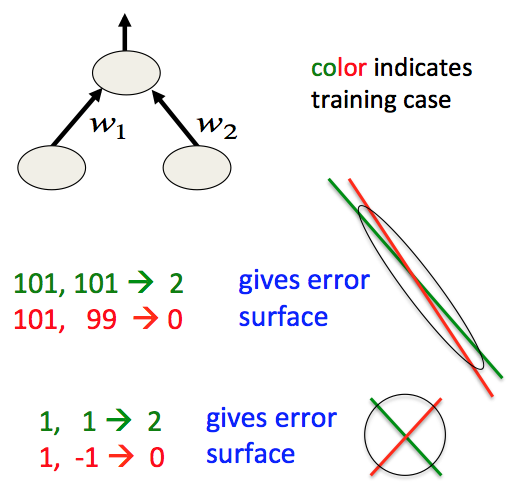
\includegraphics[width=5cm]{pics/2-inputshift.png}
\end{column}
\end{columns}
\end{frame}


\begin{frame}
\frametitle{scaling the inputs}
\begin{columns}
\begin{column}{6cm}
When using steepest descent, scaling the input values makes a big difference.
\begin{itemize}
\item It usually helps to transform each component of the input vector so that it has unit variance over the whole training set.
\end{itemize}
\end{column}
\begin{column}{5cm}
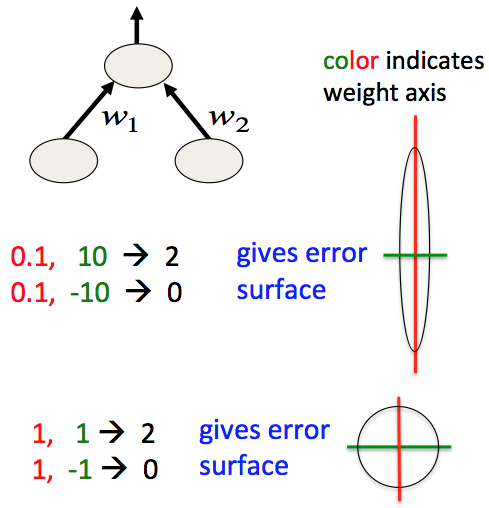
\includegraphics[width=5cm]{pics/2-inputscale.png}
\end{column}
\end{columns}
\end{frame}




\begin{frame}
\frametitle{A more thorough method: Decorrelate the input components}
For a linear neuron, we get a big win by decorrelating each component of the input from the other input components.

There are several different ways to decorrelate inputs. A reasonable method is to use Principal Components Analysis (PCA).
\begin{itemize}
\item  Drop the principal components with the smallest eigenvalues.
\item  Divide the remaining principal components by the square roots of their eigenvalues. For a linear neuron, this converts an axis aligned elliptical error surface into a circular one.
\end{itemize}
For a circular error surface, the gradient points straight towards the minimum.

\end{frame}



\begin{frame}
\frametitle{speed-up tricks}
If we start with a very large learning rate, weights get very large and one suffers from ``saturation'' in the neurons.  This leads to a vanishing gradient, and learning is stuck.

\vskip5mm
Furthermore,
\begin{enumerate}
\item use momentum (this will be explained in the ``optimisation'' lecture);
\item use separate learning rates per parameter;
\item rmsprop;
\item use a second-order method (also here, see the ``optimisation'' lecture).
\end{enumerate}
\end{frame}



%\begin{frame}
%\frametitle{the momentum method}
%\begin{columns}
%\begin{column}{6cm}
%$$\bfu(t) = \beta \bfu(t-1) - \alpha {\partial E\over\partial \bfw}(t)$$
%\end{column}
%\begin{column}{5cm}
%The effect of the gradient is to increment the previous velocity. The velocity also decays by $\beta$ which is slightly less than 1.
%\end{column}
%\end{columns}
%\vskip1cm
%\begin{columns}
%\begin{column}{6cm}
%\begin{eqnarray*}
%\Delta\bfw(t) &=& \bfu(t)\\
%&=&  \beta \bfu(t-1) - \alpha {\partial E\over\partial \bfw}(t) \\
%&=&  \beta \Delta\bfw(t-1) - \alpha {\partial E\over\partial \bfw}(t) 
%\end{eqnarray*}
%\end{column}
%\begin{column}{5cm}
%The weight change is equal to the current velocity.
%
%The weight change can be expressed in terms of the previous weight change and the current gradient.
%\end{column}
%\end{columns}
%
%\end{frame}
%




%\begin{frame}
%\frametitle{the behaviour of the momentum method}
%$$\bfu(t) = \beta \bfu(t-1) - \alpha {\partial E\over\partial \bfw}(t)$$
%$$
%\bfu(\infty) = {1\over 1-\beta} \left(-\alpha {\partial E \over \partial \bfw}\right)
%$$
%
%If the momentum $\beta$ is close to 1, this is much faster than simple gradient descent.
%
%At the beginning of learning there may be very large gradients.
%\begin{itemize}
%\item So it pays to use a small momentum (e.g., 0.5).
%\item Once the large gradients have disappeared and the weights are stuck in a ravine the momentum can be smoothly raised to its final value (e.g.\ 0.9 or even 0.99)
%\end{itemize}
%This allows us to learn at a rate that would cause divergent oscillations without the momentum.
%
%\end{frame}





\begin{frame}
\frametitle{separate adaptive learning rates}
In a multilayer net, the appropriate learning rates can vary widely between weights:
\begin{itemize}
\item  The magnitudes of the gradients are often very different for different layers, especially if the initial weights are small.
\item  The fan-in of a unit determines the size of the ``overshoot'' effects caused by simultaneously changing many of the incoming weights of a unit to correct the same error.
\end{itemize}

So use a global learning rate (set by hand) multiplied by an appropriate local gain that is determined empirically for each weight.
\end{frame}





\begin{frame}
\frametitle{how to determine the individual learning rates}
\begin{columns}
\begin{column}{6cm}
start with a local gain of 1 for every weight.

Increase the local gain if the gradient for
that weight does not change sign.

Use small additive increases and multiplicative decreases (for mini-batch)
\begin{itemize}
\item  this ensures that big gains decay rapidly when oscillations  start.
\item If the gradient is totally random the gain will hover around 1 when we increase by plus $\delta$ half the time and decrease by times $1-\delta$ half the time
\end{itemize}
\end{column}
\begin{column}{5cm}
$$\Delta w_{ij} = -\alpha g_{ij} {\partial E\over \partial w_{ij}}
$$
if $\Bigl(  {\partial E\over \partial w_{ij}}(t)  {\partial E\over \partial w_{ij}}(t-1) \Bigr) > 0$
\vskip5mm
then $g_{ij}(t) = g_{ij} (t-1) + 0.05$
\vskip5mm
else $g_{ij}(t) = g_{ij} (t-1) \cdot 0.95$
\end{column}
\end{columns}
\end{frame}







\begin{frame}
\frametitle{rprop: using only the sign of the gradient}
The size of the gradient can be very different for different weights and can change during learning.  Also remember the condition of the Hessian.
\begin{itemize}
\item  This makes it hard to choose a single global learning rate.
\end{itemize}
Idea: use only the sign of the gradient.
\begin{itemize}
\item  The weight updates are all of the same magnitude.
\item This escapes from plateaus with tiny gradients quickly.
\end{itemize}
\pause
rprop: This combines the idea of only using the sign of the gradient with the idea of adapting the step size separately for each weight.
\begin{itemize}
\item  Increase the step size for a weight multiplicatively (e.g.\ times 1.2) if the signs of its last two gradients agree.
\item Otherwise decrease the step size multiplicatively (e.g.\ times 0.5).
\item Don't make the step size too large or too small.
%\item (Rule of thumb: Limit the step sizes to be less than 50 and more than a millionth (Mike Shuster's advice)).
\end{itemize}
\end{frame}



\begin{frame}
\frametitle{rmsprop: a mini-batch version of rprop}
rprop is equivalent to using the gradient but also dividing by the size of the gradient.

The problem with mini-batch rprop is that we divide by a different number for each mini-batch. So why not force the number we divide by to be very similar for adjacent mini-batches?

\pause
rmsprop: Keep a moving average of the squared gradient for each weight
$$
\mathrm{meanSquare}(w,t) = 0.9\, \mathrm{meanSquare}(w,t-1)
	+ 0.1 \left({\partial E \over \partial w} (t)\right)^2
$$

Dividing the gradient by $\sqrt{\mathrm{meanSquare}(w, t)}$ makes the learning work much better.
\end{frame}


\begin{frame}
\frametitle{summary of learning methods}
For small datasets (e.g., 10,000 cases) or bigger datasets without much redundancy,
use a full-batch method.
\begin{itemize}
\item conjugate gradient (with Powell restarts), LBFGS, \dots
\item adaptive learning rates, rprop, \dots
\end{itemize}
 For big, redundant datasets use mini-batches.
\begin{enumerate}
\item Try Adam, Adadelta;
\item Try rmsprop (with momentum?);
\item Try gradient descent with momentum.
\end{enumerate}
Why there is no simple recipe:
\begin{itemize}
\item Neural networks differ a lot:  Very deep networks (especially ones with narrow bottlenecks);
  Recurrent networks;  Wide shallow networks. 
\item Tasks differ a lot:
  Some require very accurate weights, some don't;
  Some have many very rare cases (e.g., words).
  \end{itemize}
  \end{frame}



\begin{frame}
\frametitle{early stopping}
Early stopping is the standard regularisation technique for MLPs. 

\vskip5mm
\centerline{\imgcrop{overtraining}{Real-world example}{0.5\textwidth}{15 15 264 208}}
\vskip5mm

\ParBeg{Note:} Typically, use about 10\% to 30\% of the data for cross-validation. 

\end{frame}
\begin{frame}[fragile]
\frametitle{early stopping recipe}
\ParBeg{Note:} You also need to reserve data for testing!  So the recipe is like this:
\vskip5mm

\begin{beamerboxesrounded}[upper=def,lower=block body,width=1.03\textwidth,shadow]{\textbf{early stopping:}}
\begin{lstlisting}[mathescape]
split the data $D$ in $D_L$, $D_X$, $D_T$
repeat
  train the network one epoch on $D_L$
  cross-validating: test network on $D_X$
until $D_X$-loss did not decrease anymore for long 
select the weights with the lowest $D_X$
testing: report the error on $D_T$
\end{lstlisting}
\end{beamerboxesrounded}

Typically we use  
 60\% for $D_L$ /
 30\% for $D_X$ /
 10\% for $D_T$.
\end{frame}



%%%%%%%%%%%  some ``new'' stuff for classifiers
\begin{frame}
\frametitle{hyperparameter optimisation}
getting the last out of your NN, you need to optimise:
\begin{itemize}
\item number of hidden layers (1, 2, 3, \dots)
\item number of hidden units (50, 100, 200, \dots)
\item type of activation function (sigmoid, tanh, rectifier, \dots)
\item learning method (adam, adadelta, rprop, \dots)
\item learning parameters
\item data set split
\item data preprocessing
\item \dots
\end{itemize}
We often start finding these by ``playing around'' with some reasonable estimates.
In the end, one often uses hyperparameter optimisation to find a good set.
Random search or Bayesian Optimisation are both viable candidates.
\end{frame}

%%%%%%%%%%%  some ``new'' stuff for classifiers

\begin{frame}
\frametitle{FFNN for classification}
Take a set of classification data $\mathcal C_0 = \{(\bfx, z=0)\}$ and  $\mathcal C_1 = \{(\bfx, z=1)\}$

If we take an FFNN with sigmoidal outputs
$$
y = \phi(a) = {1 \over 1 + \exp(-a)}
$$
we can interpret the output $y(\bfx, \bfw)$ as the conditional
probability $p(\mathcal C_0 \mid \bfx)$ while $p(\mathcal C_1 \mid \bfx) = 1-y(\bfx,\bfw)$.

\pause
But then the likelihood is a Bernoulli distribution
$$
p(t \mid \bfx, \bfw) = y(\bfx, \bfw)^z \bigl[1-y(\bfx,\bfw)\bigr]^{1-z}
$$
\pause
The negative log likelihood then leads to
$$
E(\bfw) = -\sum_{p=1}^n \Bigl\{
	z_p \log y(\bfx_p, \bfw) + (1 - z_p) \log \bigl[1 - y(\bfx_p, \bfw)\bigl]
	\Bigr\}
$$
Has been shown to lead to better results!
\end{frame}




\begin{frame}
\frametitle{use one-hot encoding}
When classifying data, use one output per class: \textsl{one-hot encoding}.

Imagine the other case.  If one encodes class 1 as $z=0$ and class 2 by $z=1$, then the continuous output is difficult to interpret. 
What does $z=0.5$ mean?

This gets even worse with 3, \dots classes.

We prefer to use a one-hot encoding!  Following the previous slide, each output encodes the likelihood of $\Vec x$ belonging to that class.

\end{frame}

\begin{frame}
\frametitle{How I train my neural network}
\begin{enumerate}
\item get and scale the data, get a neural network that I hope is too wide and too deep, but I still want it to keep it small enough to train fast.
\item train the neural network to see if it can approximate the training data.  Plot the reconstruction on your training data.  Make it overfit as well as possible.  If you don't reach that stage, make your network deeper, wider, stronger, and fiddle with adam vs adagrad vs.\ nadam vs.\ \dots the whole shebang.  If you still fail, your data or your underlying problem is wrong.
\item now that I know you can represent the data in the NN, I try to represent the underlying function in the NN.  By optimising towards the validation set.  So, make the network less strong, fiddle with activation functions, initialisation, and I add regularisation, until the results are good enough on the validation set.  Hyperparameter search may work.  If all fails, there may be too few training data.
\item If all is good, I keep my fingers crossed for the test set.  If there the results are not to my liking, I need to get more data / shuffle data better (between train and validation set).  After trying with a few different seeds, knowing that that is cheating.  In the end, I despair.
\end{enumerate}
\end{frame}

\end{document}
